\begin{figure*}
  \centering
  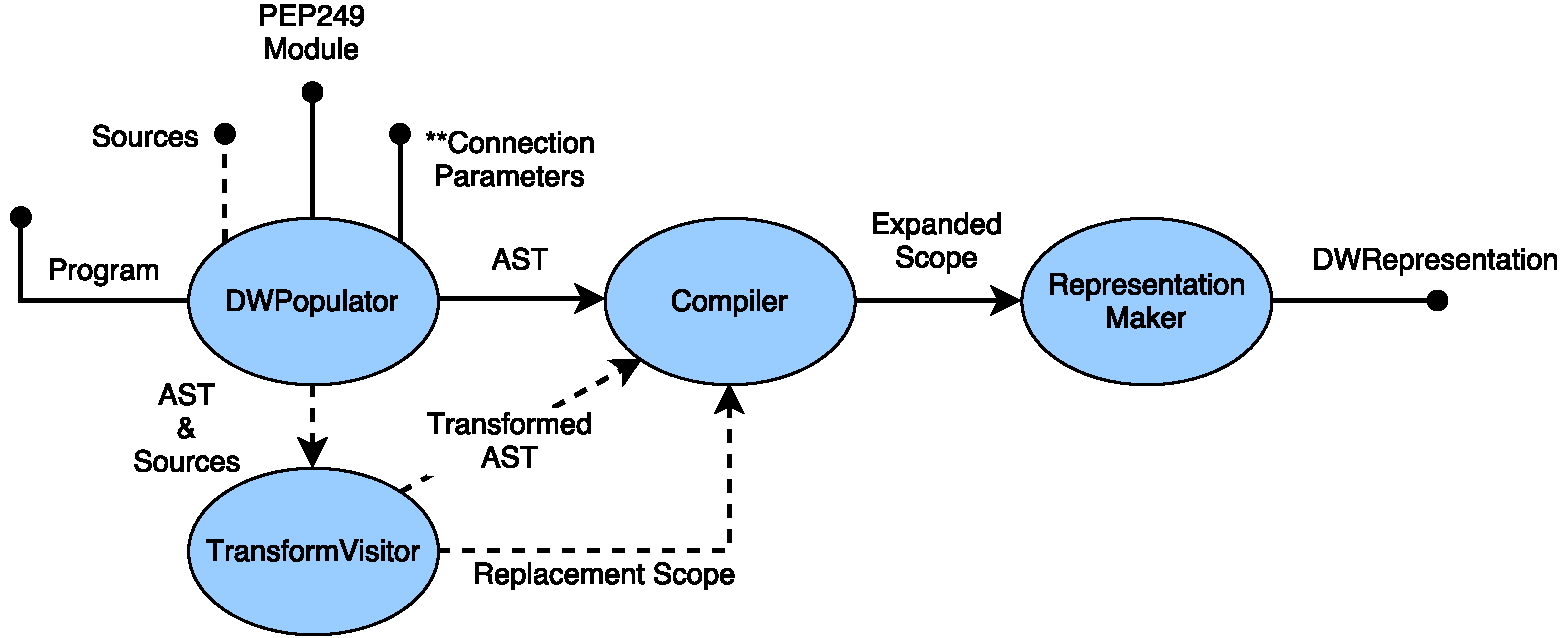
\includegraphics[width=1\textwidth]{figures/reinterpreter.pdf}
  \caption{Data flow diagraml of the Reinterpreter}
  \label{fig:reinterpreter}
\end{figure*}


\section{pygrametl Reinterpreter}


In this section we will describe, in detail, the implementation of the reinterpreter component. Its purpose is to make it easier for users to replace the sources and DW in their pygrametl programs. Users may give test sources and DW as input to the reinterpreter, rather than hardcoding them into the program itself. The reinterpreter also outputs a DWRepresentation object, which describes the structure and contents of the DW in question. On \cref{fig:reinterpreter} is a dataflow diagram which illustrates the flow of data through the reinterpreter. Please note that this depiction is abstracted from the actual implementation as to ease explanation. In the following subsections, we will describe each of the four sub-components shown on the figure. Following this we describe what restrictions the component operates according to.

\subsection{ScopeMaker}
The ScopeMaker has the job of connecting to the DW and creating the replacement scope.  The input sources are a list objects used to connect to testsources, which may either be databases or a CSV files. When connecting to a CSV file the object is a file handle, and when connecting to a database it is a PEP249 connection object. From now on, when we refer to a connection object it can be either of these two.  The component begins by first  instantiating a PEP249 connection object to the DW using the module and connection parameters. The ScopeMaker can now create the replacement scope since  connections objects to both sources and DW are avaliable, . The replacement scope is an ordered dictionary used to replace connections in the pygrametl program. Each source connection object is paired with the key \_\_x\_\_ , where x is the source's index in list plus one.  The DW connection object is paired with the key \_\_0\_\_. Once completed the replacement scope is sent to the TransformVisitor.  

\subsection{TransformVisitor}
The TransformVisitor is a class taking as input the replacement scope and the AST of the pygrametl program being tested. This component is used to walk over the AST, replacing the program's connections with those from the replacement scope.  It  inherits from ast.NodeVisitor and overwrites the visit\_Call method. This method is called, when a call node implementing  a call to a method or function, is encountered. The overwritten method is shown below:

\insertcodefile{codeRelated/scripts/CallNode.py}{The visit\_Call method of TransformVisitor} 


The method only reacts to certain pygrametl method calls. After extracting the name of the method being called, we react if the name is contained in either ATOMIC\_SOURCES or WRAPPERS.

 ATOMIC\_SOURCES  is a list of the non-aggregate sources  SQLSource, CSVSource and TypedCVSSource. All other sources from pygrametl.sources are aggregates of these three. Thus there is no reason to react to these. If the method name is contained within ATOMIC\_SOURCES it means that a non-aggregate source is being instantiated. One of the parameters used for such an instatiation is a connection object. By replacing this with the connection object of a test source, we force the non-aggregated source to point to the test data. This means that the object can now be used to access test data, rather than the data it was hardcoded to do. The replacement itself simply consists replacing the hardcoded connection parameter with a dummy key from the replacement scope. For the first source encountered the key will be \_\_1\_\_, the second \_\_2\_\_ and so on. These will later be used as identifiers, when executing the AST. 

WRAPPERS contains only ConnectionWrapper from pygrametl.init. This is the class used to access DWs. Once the instantiation of a ConnectionWrapper is encountered we simply replace its connection parameter with the key \_\_0\_\_, pointing to the test DW in the replacement scope. We also set a flag that makes sure that we raise an exception if another ConnectionWrapper is encountered. We do this to restrict \FW{} to only work with pygrametl programs that function on a single DW.

Once the entire tree has been walked a transformed AST has been produced, where we access test data instead of the one hardcoded into the program. This tree along with the replacement scope is now sent to compilation. 


\subsection{Compiler}
This is a call to the python compiler, which executes the transformed AST using the replacement scope as its local scope. In python, a scope is given by a dictionary, where keys are variable names paired with object references. As we replaced the connecting objects in the transformed AST with keys from our own scope, we force the program to use the test objects in the replacement scope. This way, we overwrite the hardcoded sources and DW from the program.  Once the AST has been executed, the test DW will be populated, and the replacement scope expanded with the variables found in the script. The expanded scope is sent to the RepresentationMaker. 

\subsection{RepresentationMaker} 
Using the expanded scope, the RepresentationMaker gains access to the Dimension and FactTable objects found within the pygrametl program. These contain a lot of useful information about each table within the DW, such as table names and keys. As database access with pygrametl is done through a PEP249 connection, meta data like this is not easily accessed. Therefore, we use these classes to get a hold of the available meta data. For each atomic Dimension and FactTable object found, we instantiate a DimensionRepresentation or FactTableRepresentation. Again, by atomic we mean that these objects connect directly to a table found in the DW. Each representation object has the purpose of storing meta data and providing access to a specific table. 

Once all tables have been found, we use them to instantiate a DWRepresentation object. This represents the entire DW, and through it all tables can be accessed. During instantiation it also computes and stores the structure of the DW based on primary/foreign key pairs between fact tables and dimensions.  pygrametl requires that a natural join can be made between tables that reference each other. Therefore we base the structure upon matching attribute names between fact tables and dimensions. Once the DWRepresentation object has been instantiated, it is returned from the reinterpreter. The DWRepresentation object is heavily used by the predicates.